\documentclass[12pt,a4paper]{article}

\usepackage{style2017}
\newcounter{numexo}
\setcellgapes{1pt}

\begin{document}


\begin{NSI}
{Activité}{Fonctionnement d'un réseau}
\end{NSI}



\section*{Les interfaces réseau}
Sur votre machine, ouvrir la page \textbf{Paramètres} puis la rubrique \textbf{réseau et internet}. 

Ensuite, afficher les propriétés du matériel et de la connexion.
\begin{enumerate}
\item De combien d'interfaces réseau votre machine dispose-t-elle ? 

Quelles sont leurs noms et leurs description ? \vspace{4cm}

\item Pour chaque interface, relever leur adresse physique et leur adresse IPv4. \vspace{4cm}

\item Comment est notée l'adresse physique d'une interface réseau ?\vspace{4cm}

\item Comment est notée l'adresse IPv4 d'une interface réseau ? et l'adresse IPv6 ? \vspace{4cm}

\end{enumerate}

\newpage
\section*{L'architecture réseau}
Dans le lycée, dans la classe, les machines sont reliées entre elles et sont connectées à internet.

\begin{enumerate}
\item Comment les machines de la classe sont-elles reliées physiquement pour communiquer entre elles ? \vspace{5cm}

\item Les machines sont reliées à internet. Qu'est-ce que ça signifie et comment est-ce possible ? \vspace{5cm}

\item À quoi sert une adresse IP ? \vspace{4cm}

\item Les adresses IP des machines de la classe se ressemblent. Pourquoi et comment s'y retrouver ? \vspace{2cm}

\item Un réseau est identifié par une adresse réseau. Pour la connaître, il faut effectuer un \& logique en binaire entre une adresse IP du réseau et le masque de sous-réseau.

Quelle est l'adresse du réseau ?

\end{enumerate}


\newpage
\section*{Communication entre 2 machines}

Les machines du lycée peuvent communiquer en s'échangeant des données et accédant à des sites web. Pour étudier la communication entre les machines, on va réaliser un réseau local avec le logiciel Filius.

\begin{enumerate}
\item Réaliser la liaison entre 2 portables comme sur la figure ci-dessous:

\begin{center}
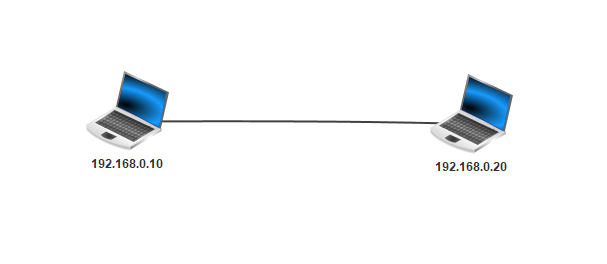
\includegraphics[scale=1]{img/reseau_1.eps}
\end{center}

\begin{enumerate}
\item Afficher les bureaux de chaque portable.
\item Ajouter sur le portable en .10 les logiciels ligne de commande et client générique.
\item Ajouter sur le portable .20 les logiciels ligne de commande et serveur générique.
\end{enumerate}
\item Le programme \textbf{ping} s'exécute en ligne de commande et prend en paramètre une adresse IP. Elle permet de vérifier la communication entre les machines.
\begin{itemize}
\item Vérifiez que vos machines communiquent avec un \textsf{ping}.
\item Afficher les échanges de données entre les deux portables.
\end{itemize} \vspace{4cm}

\newpage
\item Exécutez les logiciels client et serveur générique. Surveillez les échanges de données entre les deux portables.
\begin{itemize}
\item Démarrez le serveur générique.
\item Saisir l'adresse IP du serveur dans le client et connectez le client.
\end{itemize} \vspace{6cm}

\item Envoyez un message au serveur et observez les échanges de données. \vspace{6cm}

\end{enumerate}


\section*{Communication internet}

\begin{enumerate}
\item Ajouter un troisième portable pour qu'il communique avec les deux autres. Vérifier que les trois machines communiquent bien.
\item Ajouter un ordinateur (serveur) dont l'adresse IP est 10.0.1.2 .
\begin{enumerate}
\item Les portables et le serveur ne peuvent pas communiquer. Pourquoi ? \vspace{2cm}
\item Quelles modifications faut-il ajouter pour que les portables et le serveur communiquent ? Effectuez les changements et vérifier.
\end{enumerate}
\end{enumerate}

\end{document}

